%%%
% set up document type
%%%
\documentclass[12pt]{article}

%%%
% declare all packages
%%%
\usepackage[left=25mm, top=20mm, right=25mm, bottom=30mm,nohead,nofoot]{geometry} 

\usepackage[T2A]{fontenc}
\usepackage[utf8]{inputenc}
\usepackage[english, russian]{babel}

\usepackage{graphics, graphicx}

\usepackage{url}
\usepackage{hyperref}

\usepackage{amssymb,latexsym} 
\usepackage{MnSymbol}
\usepackage{mathrsfs}

\usepackage[nottoc,numbib]{tocbibind}
\usepackage{float}
\usepackage{listings}
\usepackage{multirow}
\usepackage{hhline}
\usepackage{delarray}

\usepackage{color,colortbl}

% \usepackage{verbatim}
%%%
% document settings
%%%
\setcounter{tocdepth}{4}
\graphicspath{ {./pic/} }

\renewcommand{\listoffigures}{\begingroup  % add number to list of graphics
\tocsection
\tocfile{\listfigurename}{lof}
\endgroup}
\renewcommand{\listoftables}{\begingroup  % add number to list of tables
\tocsection
\tocfile{\listtablename}{lot}
\endgroup}

%******************************************************************
%******************************************************************
\begin{document}

\begin{titlepage}
	\center
		Санкт-Петербургский Политехнический 
		университет \\ Петра Великого\\
		Институт прикладной математики и механики
		\\ \textbf{Высшая школа прикладной математики и вычислительной физики}

	\vfill ~
	\textbf{
		\\ \large ЛАБОРАТОРНАЯ РАБОТА №2
	}
	\\	на тему 
	\\ "Исследование разностных схем для параболических уравнений"
	\\ по дисциплине
	\\ "Конечно-разностные и сеточные методы"

	\vfill ~

	Выполнил студент гр. \textbf{3630102/60101} \\
	\textbf{Лансков.Н.В.} \\ 

\vfill

{\large}	Санкт-Петербург
\\ 2019
\end{titlepage}

%%%
% Table of conetnts 
%%%

\tableofcontents 
\newpage
\listoffigures
\newpage
\listoftables
\newpage

%%%
% Text
%%%
\section{Постановка задачи}

Рассмотрим задачу :

$$
\begin{cases}
\dfrac{du}{dt} - \rho(x)\dfrac{d^2u}{dx^2} = f(x, t), & x \in [0.5;2],  t \in [0, T] \\ \\
0 < \rho_{min} < \rho(x) < \rho_{max}, & \rho(x) = (x+1)*10^{-7} \\ \\
 - \dfrac{du}{dx}(0.5) + u(0.5) = \mu_1(t) \\ \\
\dfrac{du}{dx}(2) + u(2) = \mu_2(t) \\ \\
u(x, 0) = \phi(x)
\end{cases}
$$

Где:
$$
\begin{cases}
f(x, t) = -3sin(e^x)xe^{-3t} - x(2e^{-3t+x}cos(e^x)+e^x(cos(e^x) - e^xsin(e^x)))  \\  \\ 
\mu_1(t) = -(e^{-3t}sin(e^{0.5}) + e^{0.5}cos(e^{0.5})(0.5e^{-3t}+1))+sin(e^{0.5}(0.5e^{-3t}+1)))\\ \\
\mu_2(t) = (e^{-3t}sin(e^{2}) + e^{2}cos(e^{2})(2e^{-3t}+1))+sin(e^{2}(2e^{-3t}+1))) \\ \\
\phi(x) = (x+1)*sin(e^x)
\end{cases}
$$

Решение ищем в виде : 
$$
\begin{cases}
u^*(x) = v(x, t)w(x) \\ \\
w(x) = sin(e^x) \\ \\
v(x, t) = x*e^{-3t}+1
\end{cases}
$$ 


\section{Разностные схемы}
\subsection{Явная схема}
Для начала введём сетки по $x$ и по $t$ соответственно.
$$
\omega_h = \{x_i = a + ih, i \in \overline{0,N}, h = \dfrac{b - a}{N}\} 
$$
$$
\omega_\tau = \{t_i = i\tau, i \in \overline{0,K}, \tau K = T \} 
$$

\begin{figure}[h]
\begin{center}
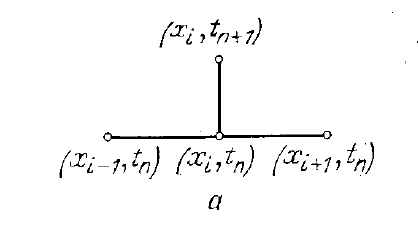
\includegraphics[scale = 0.8]{exp.png} 
\end{center}
\caption{Шаблон для явной схемы}
\end{figure}


Рассмотрим процесс нахождения значений сеточной функции. Сначала заполняем значения на нулевом слое, подставляя значения функции из начального условия $u(x, 0) = \phi(x)$. Далее для слоя с номером $n \in [1; T]$ вычисляем значения внутренних точек по схеме:
$$
\begin{cases}
y_i^n = y_i^{n-1} + \tau*(f_i^{n-1} + \rho(x_i)*y_{x\overline{x}, i}^{n-1}) \\ \\ 
y_{x\overline{x}, i}^{n-1} = \dfrac{y_{i+1}^{n-1} - 2y_i^{n-1} + y_{i-1}^{n-1}}{h^2}
\end{cases}
$$

После этого вычисляем значения в граничных точках, пользуясь граничными условиями:
$$
y_0^n = \dfrac{\mu_1(t^n) + \dfrac{4y_2^n - y_3^n}{2h}}{1 + \dfrac{3}{2h}} ; y_N^n = \dfrac{\mu_2(t^n) + \dfrac{4y_{N-1}^n - y_{N-2}^n}{2h}}{1 + \dfrac{3}{2h}} 
$$
Заметим, что производные в граничных условиях аппроксимируются по трёхточечному шаблону с порядком точности $O(h^2)$.

\subsection{Неявная схема}

\begin{figure}[h]
\begin{center}
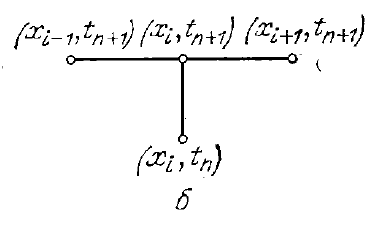
\includegraphics[scale = 0.8]{imp.png} 
\end{center}
\caption{Шаблон для неявной схемы}
\end{figure}

Неявная схема, в отличие от явной, для нахождения значений функции на одном слое требует решения трёхдиагональной системы методом прогонки.
В данной работе был реализован общий вид данной схемы.

Шаблоны по $x$ и по $t$ задаются аналогично, также аналогично первый слой заполняется при помощи начального условия.

Пусть мы заполнили $n-1$ слой, рассмотрим матрицу, которая получается на $n-ом$ шаге.

$$
\left(\begin{array}{ccccc|c}
	3+2h & -4 &  1 & 0 & ... & 2h\mu_1(t_n) \\
	\gamma_1 & -1-2\gamma_1 & \gamma_1 & 0 & ... & -(y_1^{n-1} + \tau (f(x_1, t_{n-1}) + \rho(x_1) (1-\sigma) y_{x\overline{x}, 1}^{n-1} )) \\
	0 & \gamma_2 & -1-2\gamma_2 & \gamma_2 & ... & -(y_2^{n-1} + \tau (f(x_2, t_{n-1}) + \rho(x_2) (1-\sigma) y_{x\overline{x}, 2}^{n-1} )) \\
	... & ... & ... & ... & ... &  ... \\
	... & 0 & \gamma_{N-1} & -1-2\gamma{N-1} & \gamma_{N-1} & -(y_{N-1}^{n-1} + \tau (f(x_{N-1}, t_{n-1}) + \rho(x_{N-1}) (1-\sigma) y_{x\overline{x}, N-1}^{n-1} )) \\
	... & 0 & 1 & -4 & 3+2h & 2h\mu_2(t_n) 
\end{array}\right)
$$
Где:
$$
\gamma_i = \dfrac{\tau \rho(x_i) \sigma}{h^2}, i \in \overline{1, N-1}
$$

Эта система строится для каждого слоя, затем приводится к трёхдиагональному виду и решается методом прогонки. 
Также в выражениях для коэффициентов фигурирует $\sigma$. Для чисто неявной схемы считаем $\sigma=1$ 

\newpage
\subsection{Симметричная схема}

Вычисления для симметричного шаблона производятся точно также, как и для случая неявной схемы, однако в данном случае $\sigma = \dfrac{1}{2}$. 

\begin{figure}[h]
\begin{center}
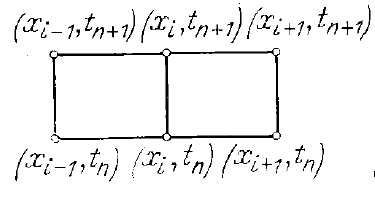
\includegraphics[scale = 0.8]{sym.png} 
\end{center}
\caption{Шаблон для симметричной схемы}
\end{figure}

\section{Результаты}
\subsection{Явная схема}
\subsection{Неявная схема}
\subsection{Симметричная схема}
\subsection{Сравнение трудоёмкости схем}

Трудоёмкость схем будем сравнивать по времени работы. Ниже приведена сводная таблица для трёх схем.

\section{Выводы}

\section{Приложения}
Исходные файлы лабораторной работы можно найти тут: \\
\url{https://github.com/LanskovNV/numerical-analysis/tree/master/%D0%A1%D0%B5%D1%82%D0%BE%D1%87%D0%BD%D1%8B%D0%B5%20%D0%BC%D0%B5%D1%82%D0%BE%D0%B4%D1%8B/lab_2}
\end{document}

